\section{Basics of visulatization}



\subsection{How to plot in Python}

\begin{frame}{Main libraries}
  
\begin{description}
\item[matplotlib] The workhorse and underlying basic of most of the following packages
\item[seaborn] More fancy, compromosie between Pythonic
\item[plotnine] An attempt to implement R ggplot2 in Python
\item[plotly] Fancy plots, support interactivity
\item[bokeh] Powerful interactive visualizations
\end{description}

\pause

You really should know matplotlib and seaborn (because they are so common), the rest is optional. For your final project, use whatever you want.

\end{frame}




\begin{frame}[fragile]{Two interfaces to Matplotlib}
  Two ways to produce this graph:
  
  \centering
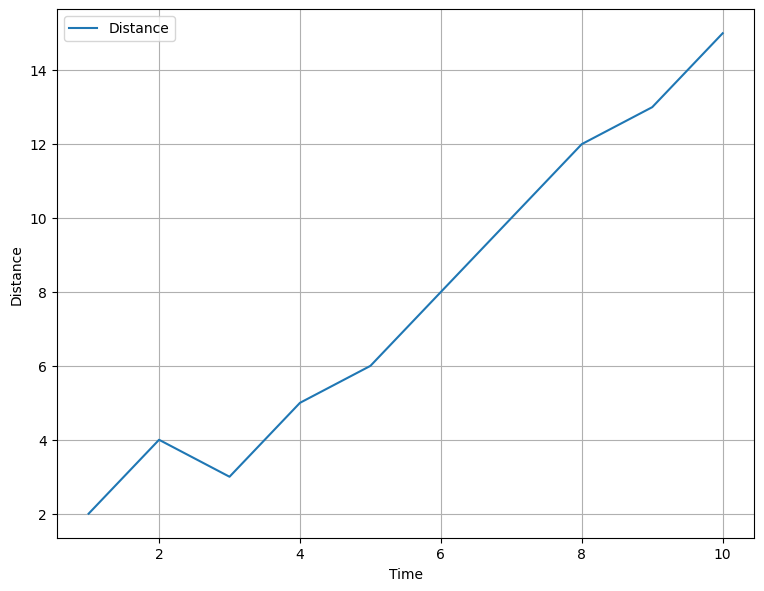
\includegraphics[width=.5\linewidth]{matplotlib01.png}\hfill


\tiny inspired by \url{https://matplotlib.org/matplotblog/posts/pyplot-vs-object-oriented-interface/}


\end{frame}



\begin{frame}[fragile]{Matplotlib: Pyplot (MATLAB inspired interface)}
(1) Building up the plot line-by-line
  
\begin{minted}{python}
import matplotlib.pyplot as plt

x = [1,2,3,4,5,6,7,8,9,10]
y = [2,4,3,5,6,8,10,12,13,15]

plt.figure(figsize=(9,7), dpi=100)
plt.plot(x,y)
plt.xlabel("Time")
plt.ylabel("Distance")
plt.legend(["Distance"])
plt.grid(True)
\end{minted}

 
\end{frame}


\begin{frame}[fragile]{Matplotlib: Object-oriented interface}
(2) Creating and motifying objects
\begin{minted}{python}
fig, ax = plt.subplots()

ax.set_ylabel("Distance")
ax.set_xlabel("Time")
ax.plot(x, y, "blue")
ax.xaxis.grid()
ax.yaxis.grid()

fig.set_size_inches(9,7)
fig.set_dpi(100)
\end{minted}

\end{frame}


\question{Can you think of pros and cons?}

\begin{frame}{Matplotlib: Two interfaces}
  \begin{itemize}
  \item You will find examples using both styles
  \item Pyplot: can be shorter/quicker/easier
  \item OO: because you get named objects, you can modify them/refer to them/etc:
  \end{itemize}

  \pause

  ``Also, the pyplot approach doesn't really scale when we are required to make multiple plots or when we have to make intricate plots that require a lot of customisation. However, internally matplotlib has an Object-Oriented interface that can be accessed just as easily, which allows to reuse objects.''

  \tiny \url{https://matplotlib.org/matplotblog/posts/pyplot-vs-object-oriented-interface/}
  
\end{frame}


\begin{frame}{Pandas and Plotting}
  \begin{itemize}
  \item As we have seen, we can directly plot from lists
  \item But if we have a dataframe \emph{anyway}, we can:
    \begin{itemize}
    \item use the build-in \texttt{.plot()} method to have pandas handle the (default: matplotlib) backend; or
    \item use seaborn directly on the dataframe
    \end{itemize}
  \end{itemize}
\end{frame}

\begin{frame}[standout]
Let's look at INSERT NOTEBOOK HERE for a demonstration
\end{frame}
